\documentclass[12pt,fleqn]{article}

\usepackage[utf8]{inputenc}
\usepackage[T2A]{fontenc}
\usepackage{amssymb,amsmath,mathrsfs,amsthm}
\usepackage[russian]{babel}
\usepackage[pdftex]{graphicx}
\usepackage{multirow}
\usepackage[footnotesize]{caption2}
\usepackage{indentfirst}
\usepackage[colorlinks,linkcolor=blue(ryb),citecolor=blue(ryb), unicode]{hyperref}

\usepackage{xcolor}
\usepackage{sectsty}

\definecolor{blue(ryb)}{rgb}{0.01, 0.28, 1.0}
%\usepackage[ruled,section]{algorithm}
%\usepackage[noend]{algorithmic}
%\usepackage[all]{xy}

% Параметры страницы
\textheight=24cm % высота текста
\textwidth=16cm % ширина текста
\oddsidemargin=0pt % отступ от левого края
\topmargin=-2.5cm % отступ от верхнего края
\parindent=24pt % абзацный отступ
\parskip=0pt % интервал между абзацам
\tolerance=2000 % терпимость к "жидким" строкам
\flushbottom % выравнивание высоты страниц
%\def\baselinestretch{1.5}
\setcounter{secnumdepth}{0}
\renewcommand{\baselinestretch}{1.1}

\newcommand{\norm}{\mathop{\rm norm}\limits}
\newcommand{\real}{\mathbb{R}}

\newcommand{\ex}{\mathbb{E}}
\newcommand{\diag}{\mathrm{diag}}
\newcommand{\intset}{\mathrm{int}}
\newcommand{\softmax}{\mathop{\rm softmax}\limits}
\newcommand{\lossfunc}{\mathcal{L}'}
\newcommand{\elbo}{\mathcal{L}}
\newcommand{\normal}[3]{\mathcal{N}(#1 | #2, #3)}
\newcommand{\dd}[2]{\frac{\partial#1}{\partial#2}}
\newcommand{\kl}[2]{\mathop{KL}(#1 \parallel #2)}
\newcommand{\nm}{\mathcal{N}}
\newcommand{\sle}{\; \Rightarrow \;}
\newcommand{\indpos}{\mathbf{I}_{d_k}^{+}[i, j]}
\newcommand{\indneg}{\mathbf{I}_{d_k}^{-}[i, j]}

\usepackage{pgfplots}

%my settings
\graphicspath{{../figures/}}
\usepackage{wrapfig}

\title{Библиотека для визуализации графика в параллельных осях}

\author{Тыцкий Владислав}
\date{Ноябрь 2020}

\begin{document}

\maketitle
\section{Графики в параллельных осях}
График в параллельных осях --- метод визуализации многомерных данных.

Для отображения векторов в n-ом пространстве рисуется n параллельных линий(осей) на равном расстоянии друг 
от друга. Вектор представляется в виде ломаной кривой, с вершинами на параллельных осях. Точка пересечения
линии с i-ой осью соответствует i-ой координате объекта.

\begin{wrapfigure}[9]{r}{0.4\textwidth}
    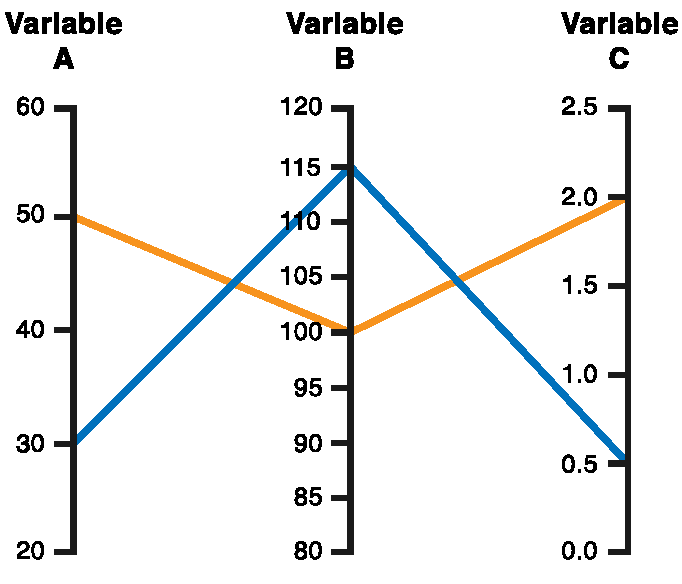
\includegraphics[width=0.9\linewidth]{parallel_coordinates.pdf} 
    \caption{Пример графика}
    \label{parallel_coords}
\end{wrapfigure}
Возникают естественные вопросы:
\begin{itemize}
    \item В каком порядке расположить оси?
    \item В какую сторону направлять ось?
    \item Какой масштаб выбрать для каждой оси?
\end{itemize}
Существуют программные реализации графики в параллельных осях: ELKI, GGobi, Mondrian,
Orange, ROOT, plotly.

К своему удивлению обнаружил, что в matplotlib из коробки нет parallel coordinates. Его можно построить только
с пакетом pandas(внутри они все равно используют matplotlib).
\newline

\section{Иерархические графики}
При визуализации большого количества объектов(векторов) график в параллельных осях становится сложночитаемым.
Связано это с тем, что количество линий на графике становится также много, все друг на друга наслаивается и разобраться
в этом невозможно.

Одним из методов решения этой проблемы является добавление кластеров(можно рассматривать просто метки классов) ---
каждому кластеру(классу) соответствует определенный цвет, и каждый объект окрашивается в цвет кластера(класса).
Такой подход немного помогает, но можно обобщить эту идею до более сложной.

\begin{figure}
    \centering
    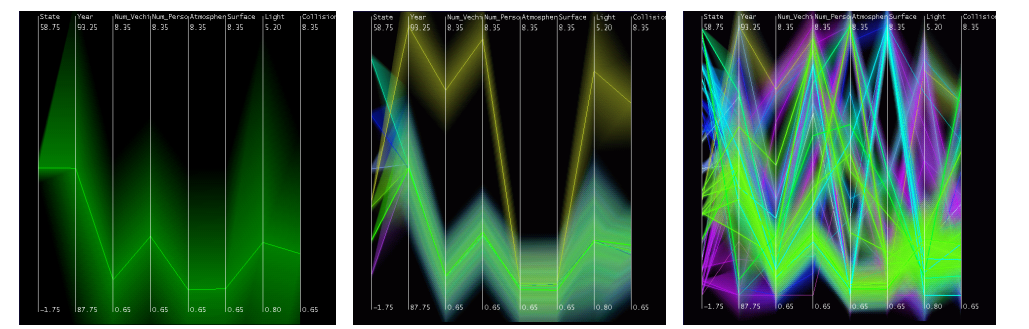
\includegraphics[width=17cm]{hierarchical.png}
    \caption{Изображения графиков начиная с корня и заканчивая большим количеством кластеров}
    \label{hierarchical_coords}
\end{figure}
Иерархические графики в параллельных осях представляют собой метод визуализации не объектов, а некоторых иерархических
кластерных структур --- дендрограмм. Давайте вместо визуализации конкретных объектов будем
визуализировать сообщества похожих объектов(меру похожести можно выбрать). Чтобы визуализировать сообщества(кластеры)
нужно выбрать некоторые статистики, например среднее и стандартное отклонение. Среднее нарисуем обычной линией, а 
стандартное отклонение отобразим полупрозрачным градиентом Рис.\ref{hierarchical_coords}. Так график становится 
более читабельным, а детализацию будем регулировать с помощью включения новых кластеров из дендрограммы.

\section{Что должно быть в библиотеке}
В библиотеке необходимо реализовать:
\begin{itemize}
    \item построение обычных графиков в параллельных осях
    \item построение иерархических графиков
    \begin{itemize}
        \item отрисовка полупрозрачного градиента(заливки)
        \item работу с иерархическими кластерами(дендрограммами)
        \item цветовое кодирование кластеров
    \end{itemize}
    \item опционально
    \begin{itemize}
        \item выделение подмножества линий в  диапазоне значений одной из осей
        \item нахождение оптимального расположения осей
        \item создание иерархических кластеров на основе входящей выборки
    \end{itemize}
\end{itemize}
\section{Эстетика в визуализации}
Помимо основных вещей, таких как легенда, подписи к осями, отметки на осях, название графика, хотелось бы добавить:
\begin{itemize}
    \item цветовые схемы
    \item плавные градиентые переходы 
    \item полупрозрачность линий
\end{itemize}
Ориентироваться можно на библиотеку \href{https://parasoljs.github.io/}{parasoljs}. Parasol современная интерактивная
библиотека для построения parallel coordinates, делающая почти все, что необходимо,
кроме отображение кластеров с помощью полупрозрачной градиентной заливки.
\section{Дизайн библиотеки}
Функционал и интерфейс библиотеки хочется сделать приближенным к более высокоуровневым библиотекам(например seaborn).

Пока не продумал прототипы функций, но можно будет за основу взять реализацию обычных графиков в параллельных осях в pandas.
\end{document}